% !Mode:: "TeX:UTF-8"

% \chapter{测试}
\section{测试2}
\subsection{subsection name子}
\subsubsection{afdf啊啊啊}
% \part{111}
\paragraph{一段文字}
\subparagraph{子段落文字}

一段文字\footnote{测试脚注},测试引用图片\upcite{RN3},如图~\ref{fig:1}
% dsad\\
%   {\chuhao 爱迪生多撒多c} \\
%   {\xiaochuhao 爱迪生多撒多xc}\\
%   {\yihao 爱迪生多撒多1}\\
%   {\erhao 爱迪生多撒多2}\\
%   {\sanhao 爱迪生多撒多3}\\
%   {\sihao 爱迪生多撒多4}\\
%   {爱迪生多撒多MR}\\
%   {\xiaosihao 爱迪生多撒多x4}\\
%   {\wuhao 爱迪生多撒多5}\\
%   {\liuhao 爱迪生多撒多6}\\
%   {\qihao 爱迪生多撒多7}
%

%
% 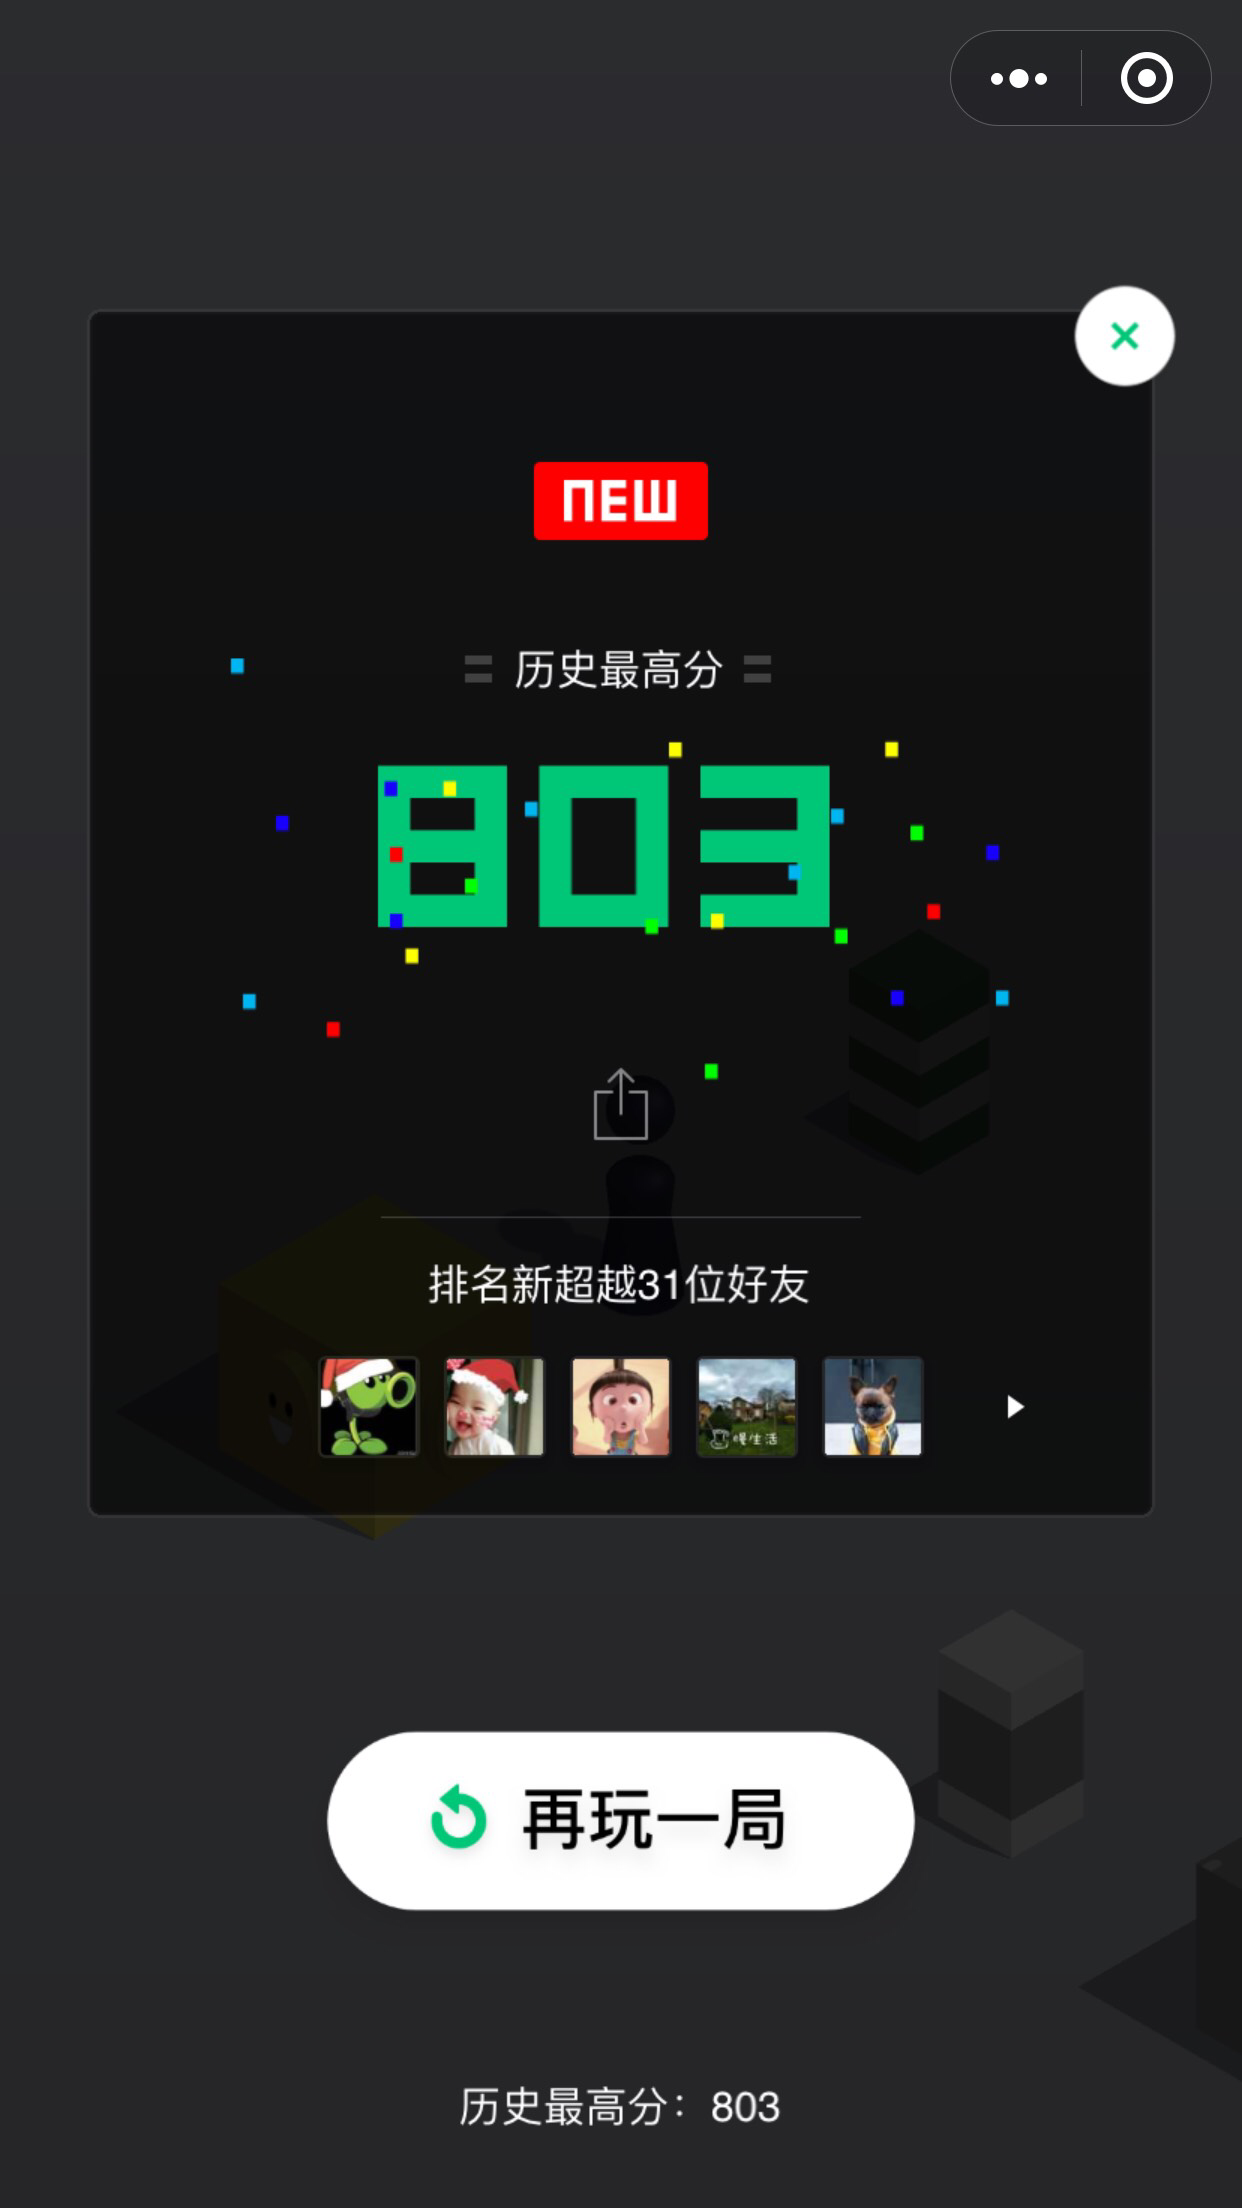
\includegraphics[height=2cm]{1.png}
%
\begin{figure}[t]
  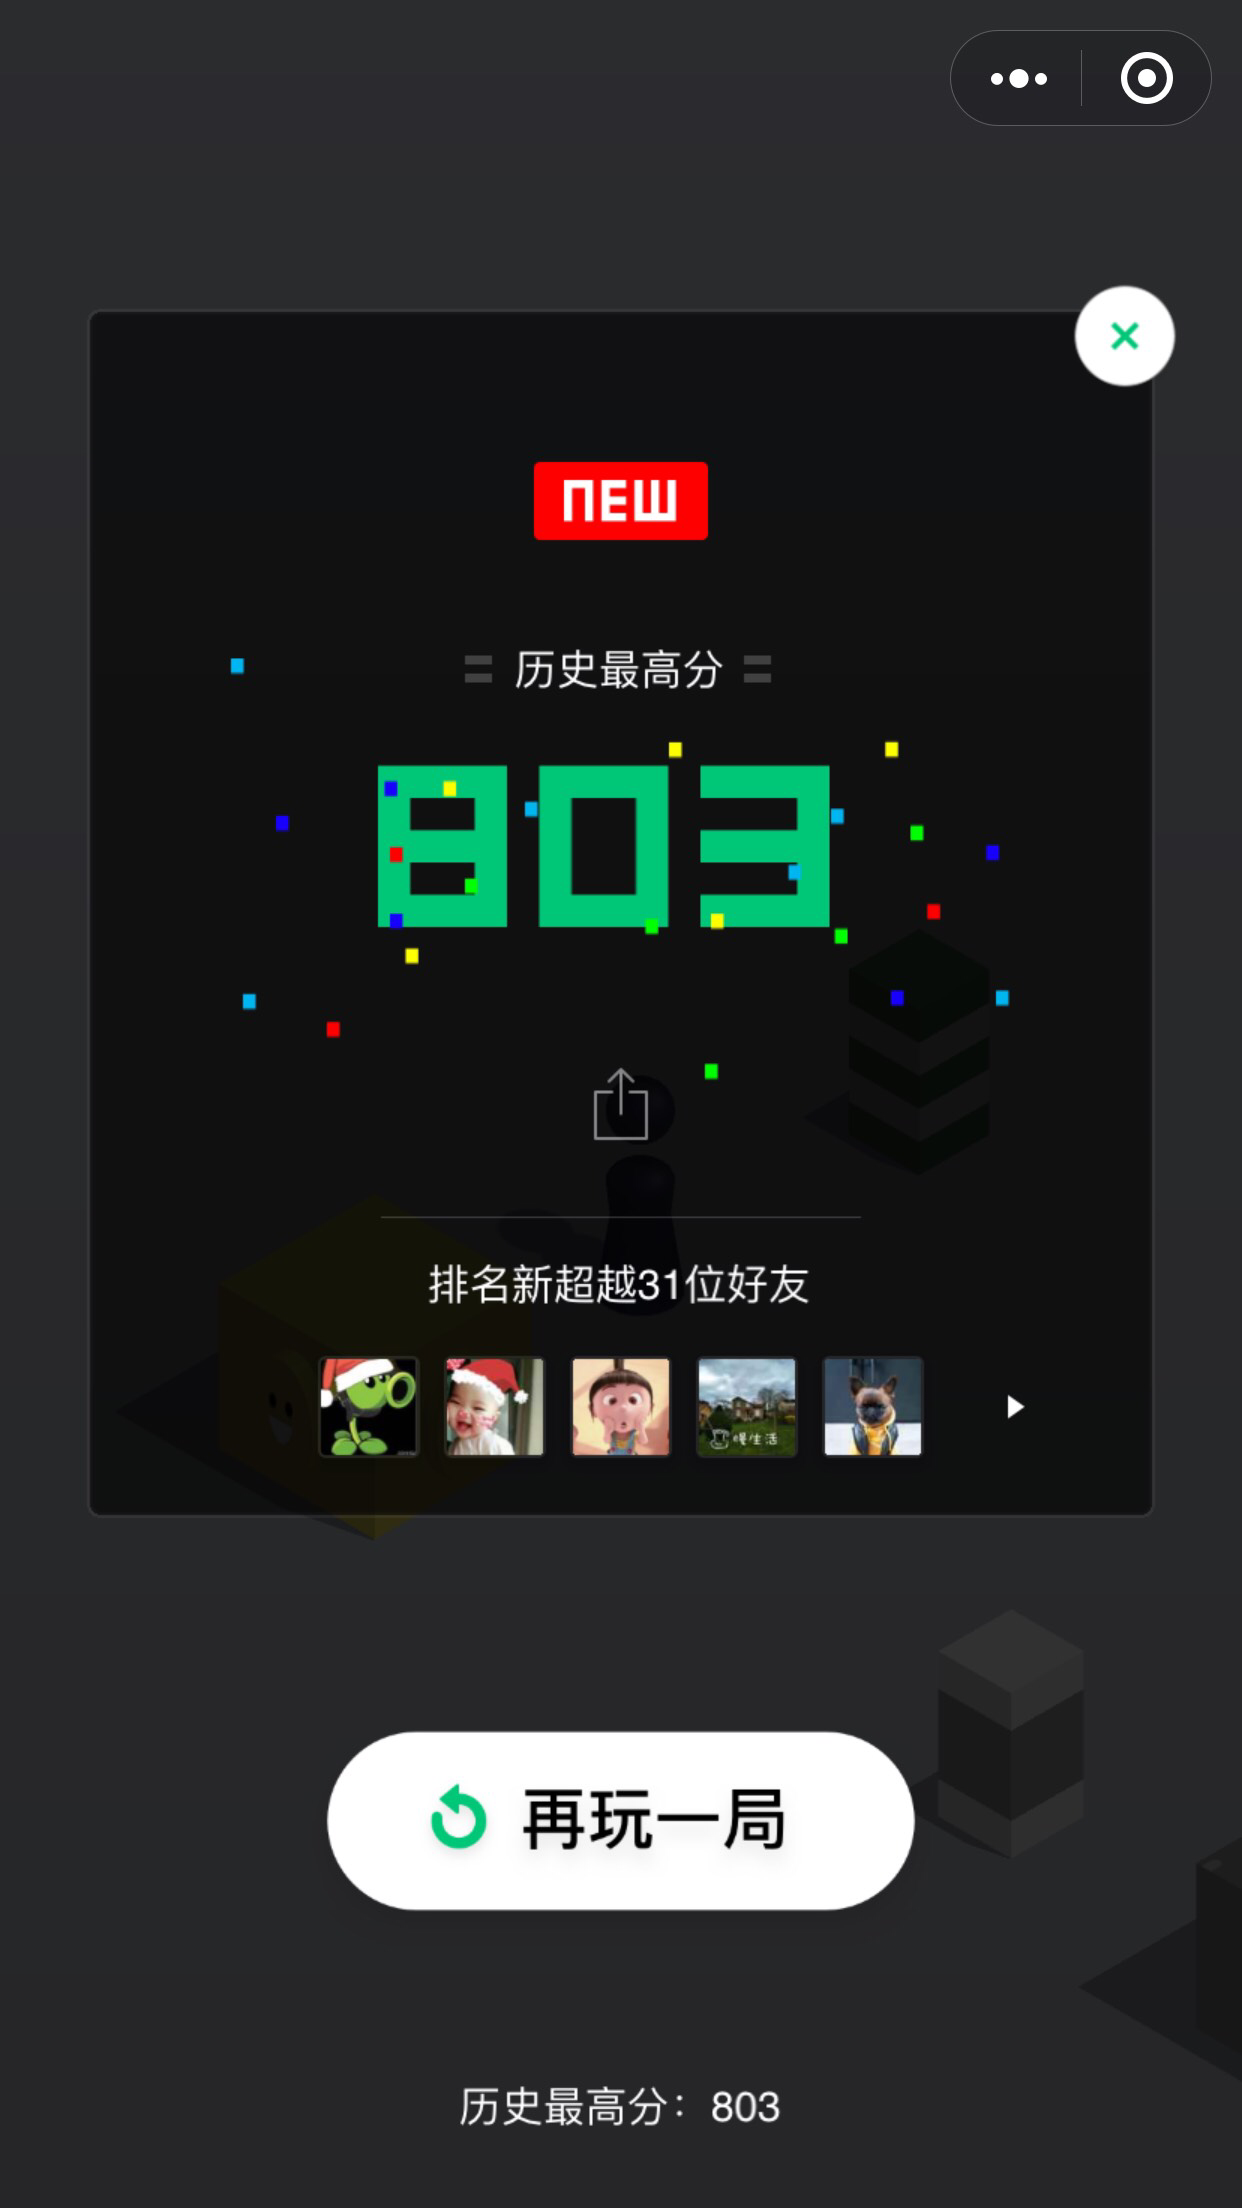
\includegraphics[height = 1 cm]{1.png}
  \caption{这是一张图}
  \label{fig:1}
\end{figure}
